\documentclass[11pt]{article}
\usepackage{framed, color}
\usepackage{textpos}
\usepackage{natbib}
\usepackage[top=1in, bottom=1in, left=1in, right=1in]{geometry}
\usepackage{color}
\usepackage{hyperref}
\usepackage{textcomp}
\usepackage{graphicx}
\usepackage{fancybox}
\usepackage{setspace}
\hypersetup{colorlinks=false, urlcolor=blue, citecolor=black}
\usepackage{soul}
\usepackage{geometry}
\usepackage{color}
\newgeometry{top=1in, bottom=1in, left=1in, right=1in}
\usepackage{fancyhdr}
\usepackage{wrapfig}
\usepackage{mdframed}
\pagenumbering{arabic}
\usepackage{fontspec}
\setmainfont{Arial}

\linespread{1.2}

\begin{document}


%\parindent 0.000000001in
\setlength{\parindent}{1cm}
\setcounter{page}{0}
\pagenumbering{arabic}

\fancyhead[CO]{Matthew D. MacManes | Research Strategy}
\pagestyle{fancy}



%\noindent \large{\textbf{\textsc{A. Personnel:}}} \\
%\normalsize 
%
%\noindent \textsc{MacManes, Matthew D} \\
%Department of Molecular, Cellular \& Biomedical Sciences. \\
%University of New Hampshire, Durham, NH 03824 USA \\
%
%\noindent
%\noindent STATUS: PI (Beginning Investigator)\\
%TITLE: Assistant Professor \\
%ROLE: Dr. Matthew MacManes will be responsible for all aspects of the project including design, collection and analysis of next-generation sequencing data, genome and transcriptome assembly, analyses of differential gene expression across experimental manipulations, generation and analysis of physiology data, supervising undergraduate and graduate students, postdocs at the University of New Hampshire, writing manuscripts, presentation of results at scientific conferences, and public outreach in New Hampshire.
%\newpage

\setcounter{page}{1}
%\noindent \large{\textbf{\textsc{2. Project:}}}
\normalsize 
\begin{center}
\textsc{{i. Significance}} \\
\end{center}

The maintenance of water balance in animals is one of the most important physiologic processes, and is critical to survival. Indeed, humans are exquisitely sensitive to changes in osmolality, with slight derangement eliciting physiologic compromise. When the loss of water exceeds dietary intake, dehydration - and in extreme cases, death - can occur. Although dehydration is both common and dangerous, a large swath of the biology underlying its physiological effects is currently invisible to researchers using traditional mammalian models of disease that lack the eco-evolutionary history present in desert-adapted mice. As such, the proposed work addresses a critical barrier (lack of an appropriate model) to the study of dehydration. In brief, which traditional models of mammalian kidney function represent powerful tools with which normal kidney function may be assayed, evolution has given us the opportunity to understand the limits of osmoregulation from a completely novel perspective. This new model has many of the benefits of traditional models,  

In addition to this, the proposed work addresses a significant question in the field 






\normalsize 
\begin{center}
\textsc{{ii. Innovation}} \\
\end{center}


I propose to study extreme physiologic water conservation using a captive colony of \textit{Peromyscus eremicus} rodents native to the desert Southwest. These rodent are housed in a specially designed walk-in desert chamber. This chamber will replicate the intense heat and aridity of the natural environment, while preserving the ability to manipulate the relevant variables (temperature, humidity, water availability) to meet experimental needs. For animals exposed to various experimental treatments (\hyperlink{Figure 1}{Figure 1}, n=10 per treatment), I will collect and analyze physiologic data relevant to hydration status (\textit{e.g.} serum electrolyte levels), and kidney function (\textit{e.g.} BUN, Creatinine). In addition to this, because water requirements are related to metabolic rates I will collect data related to metabolism using a chamber designed to function in extreme desert conditions. Lastly, though most individuals are functionally anuric, urine will be collected when available and analyzed for specific gravity and osmolality. 

In addition to the thorough characterization of physiology related to desert survival, I will characterize the genomic changes that underlie changes in physiology. To do this, I will perform carefully controlled Bisulfite and RNA sequencing experiments using renal medullary tissue to assay the genomic changes accompanying changes in physiology. These data represent a uniquely rich characterization of both the phenotype (=physiology) and genomics surrounding desert life, and will significantly enhance our understanding of desert survival. 


\begin{center}
\textsc{{ii. Background}} \\
\end{center}
The study of adaptation, or the process through which animals become fitted to their environment has intrigued researchers for decades \citep{Darwin:1859tm, Fisher:1930wy}, though only recently have we had the ability to study the underlying genomic mechanisms. Interestingly, researchers interested in understanding the genetics of adaptation have the ability to ground modern studies of genetics on decades of work aimed at understanding the ecological context within which adaptation occurs. One particularly salient example of the connection between studies of ecology and natural history and modern genomics can be found in the study of physiologic adaptation to desert conditions. Here, remarkable physiologic, morphologic \citep{Dickinson:2007jn,Huntley:1984us,SchmidtNielsen:1950wg,SchmidtNielsen:1952wp} and behavioral \citep{NAGY:1994vd} adaptation has been studied in the context of desert ecology. These studies provide a rich context for the current work, which aims to define the relationship between physiology and genomics in rodents able to thrive in amongst the most harsh of conditions on Earth.  

Though classic research relating morphology (especially renal ultrastructure) and physiology to desert adaptation has been done, we know virtually nothing about how extreme heat and aridity may affect other core physiological and metabolic processes. For instance, the maintenance of normal serum electrolyte concentration is challenging in the context of desert conditions. Indeed, electrolyte derangement is often the ultimate cause dehydration-related death, yet for the vast majority of desert animals, we know nothing of electrolyte balance - not even typical values! Understanding these critical processes is fundamental to our understanding of physiological adaptation, and will be accomplished as part of this project. 

Lastly, the genomic processes related to desert survival have yet to be characterized. The few studies of genetics that have been done have focused on the role of single members of the Aquaporin gene family (but see \cite{Bartolo:2007hy}), which are large membrane-bound proteins that are critically involved in renal water transport \citep{Kwon:2009bv,Verkman:2002ww,Brown:1995vo,Nielsen:1995cb}. These studies have shown that changes in Aquaporin (AQP) protein abundance and expression may be related to water availability \citep{Boselt:2009fb, Gallardo:2005fm,Bozinovic:2003eg}. In addition to changes in expression, another study showed that the AQP4 pathway was completely lost in the desert rodent \textit{Dipodomys merriami merriami} \citep{Huang:2001ti}. Despite these studies, we have a limited understanding of the genomics of renal water and solute regulation in desert animals. While AQPs are functionally important, water and solute balance is extraordinarily complex, and therefore single-gene studies are necessarily limited in their purview. A more complete understanding of this phenotype and its mechanistic underpinnings will require a sophisticated genome-level approach, which will be the outcome of the proposed research. 

\begin{center}
\textsc{{iii. Experimental Plan and Preliminary Results}} \\
\end{center}
\begin{wrapfigure}{r}[0pt]{0.5\textwidth}
\hypertarget{Figure 1}{}
\vspace{-5mm}
\begin{mdframed}
  \begin{center}
    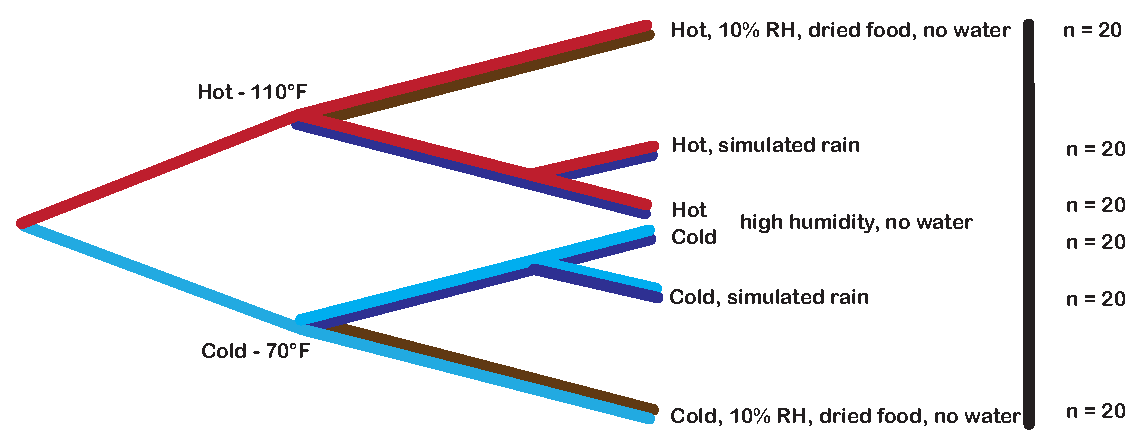
\includegraphics[width=1\textwidth]{exp_design_fig.eps}
  \end{center}
  \caption{\small{Animals are relegated into either hot or cold treatments. Within treatments (n=10 per treatment), animals are exposed to two weeks of varying levels of aridity, from simulated rainfall where water is available \textit{ad libitum}, to dry, where no water is available. RH=relative Humidity}}
\end{mdframed}
\end{wrapfigure}

\textbf{Specific Aim 1:} To better understand the physiological effects of desert conditions on rodents, \ul{I will relate multiple physiological variables to differences in temperature, relative humidity, and water availability.} These experiments (and those described under Aim 2) are fundamentally linked to a series of environmental manipulations, described in \hyperlink{Figure 1}{Figure 1}. I hypothesize that, as a result of unique mechanisms related to solute and water balance, that average electrolyte concentrations will remain relatively constant throughout various experimental manipulations, but the variance in measured levels between individuals will increase in the most extreme conditions.


From all animals in experimental treatment groups (n=10 * 6 treatments=60 animals), I will collect a urine sample, and measure specific gravity and urine osmolality using an Atago UG-$\alpha$ urine refractometer. Serum electrolytes including potassium, sodium, BUN, creatinine, calcium and bicarbonate ion concentration will be measured. Metabolic parameters including carbon dioxide production and oxygen consumption will be measured will be measured during a twelve hour period at the end of the experimental manipulation, just prior to euthanasia, using a standard metabolic chamber (Sable Inc.) modified for use in the desert chamber. 

\textsc{{Preliminary Data:}} To date, I have generated a physiology dataset that consists of serum electrolytes and urine osmolality from 5 animals housed in the 'cold/simulated rain' treatment group. This small dataset allowed me to refine and perfect the protocols for data collection and analysis, and has already suggested interesting physiology. In the small subset of animals housed in the cool, wet, simulated rain conditions for a period of 3 weeks, all had serum Potassium levels \textgreater 8.0, Creatinine \textless 0.3, and Sodium \textgreater 151, which is significantly different than 'normal' levels for other mammals.  

\textbf{Specific Aim 2:} \ul{I will understand the genetic response to extreme heat and aridity via a series of bisulfite sequencing and RNAseq experiments, and will link these patterns to individual physiologic state as defined in Aim 1.} Differences in renal methylation patterns and mRNA gene expression will be tested using the 10 individuals per treatment group (n=60 total, specified above). I hypothesize that genes responsible for water and solute transport will be particularly active in the most extreme conditions.  

For analysis of the bisulfite sequence data, an accurate genome assembly is required. Using the existing draft genome (sequenced using startup funds) as a starting point, I will complete the genome assembly of the primary study organism, \textit{Peromyscus eremicus}. This process will be significantly aided by leveraging the existing genome sequence data available from several other \textit{Peromyscus} species. Specifically, an additional 60X coverage Illumina dataset using 150bp paired end and mate-pair sequencing will supplement the current 40X dataset. Simultaneous with this, I will sequence up to 10X coverage using long-read PacBio sequencing. A short-read assembly of Illumina data will be done using AllPaths-LG \citep{Maccallum:2009du}.  Illumina contigs will be assembled with the corrected PacBio data using the software package SGA \citep{Simpson:2012ef} or an overlap-layout-consensus assembler (\textit{e.g.} Celera, \cite{Miller:2008jx}) to generate a primary \textit{de novo} genome assembly. Assemblies will be validated by use of the CEGMA \citep{Parra:2007df} and REAPR \citep{Hunt:2013hj} algorithms. In general, this approach has been shown to be successful in producing high quality draft assemblies, though multiple assembly methods will be evaluated as per the findings of my previous work \citep{Bradnam:2013gx}.

To annotate the genome, RNA and smRNA sequence data from several tissues, including liver, kidney, and brain will be generated. Sequence data will consist of Illumina strand-specific small-insert 150bp paired end sequencing. Each tissue type will be sequenced to a depth of 100 million reads.  Assembly will be accomplished using the Trinity software package \citep{Haas:2013jq,Grabherr:2011jb} after error correction \citep{MacManes:2013ec} and quality trimming \citep{MacManes:2013ex}. Annotation will be completed using the programs Trinotate (\url{http://trinotate.sourceforge.net/}) and Maker \citep{Cantarel:2008jo}. 

In addition to the assembly and annotation of the \textit{P. eremicus} genome, a secondary result of this work is methods development (\textbf{enhancing infrastructure}). To this end, I have already already released a transcriptome assembly pipeline (\url{http://sourceforge.net/projects/tamrs/}) and automated quality control software (\url{http://sourceforge.net/projects/qcpro/}). In addition to this, I am an active developer of the transcriptome assembly program Trinity and annotation software Trinotate. Given the popularity of high-throughput sequencing, the demand for these types of tool development programs will likely increase.  

\textsc{{Preliminary Data:}} To date, I have generated a RNAseq dataset that consists of approximately 30M 150nt SE Illumina reads from the same 5 animals housed in the 'cold/simulated rain' treatment group from which I collected physiology data. 

\textbf{Specific Aim 3:} Given that desert adapted mice, capable of surviving without water are as neonates dependent on liquid intake, \ul{the study of the ontogeny of physiologic water conservation is extremely interesting and relevant to the current work.} This phenomenon will be explored using neonate mice in the treatments listed in Aim 1, and methods described in Aim 2. Five neonate mice will be culled per treatment at 3 different timepoints (immediately after birth, mid-lactation, 1 day after weaning). I hypothesize that patterns of gene expression and methylation will resemble those common in conditions where water is available \textit{ab lib}.  
\begin{center}
\textsc{{iv. Broad Impacts}} \\
\end{center}
How desert animals survive without water is an intrinsically interesting example of extreme physiology and adaptation. Indeed, telling people of the remarkable story of a rodent that may never drink water is immediately captivating. Having told hundreds of people, including children, adults, scientifically literate and not, the most common response is something like "Wow! That is amazing. How do they do that?" I intend to \textbf{broaden dissemination} by capitalizing on this common response, using traditional and non-traditional methods. While lecture has been the mainstay of scientific communication, its audience tends towards the educated/affluent subset of the population. Given one of my primary goals as a scientists is to broadly share my work, I will use non-traditional modes of communication which will include social media and a blog. All publications are hosted on a public preprint server, and published using using open access options. All data and code is freely available using public repositories like Github, Dryad, or Figshare. In addition to this, I will develop an outreach program that aims to present research findings to school-aged children. These program will be multi-dimensional, with programs geared towards several different age groups. 

\textbf{Broadening participation} is an issue about which I care deeply. As a scientist of Native American descent, I strive to be a role model and mentor for underrepresented groups. To this end, I am developing an internship program- in collaboration with the American Indian Higher Education Consortium (\url{http://aihec.org/}), where qualified Native students may spend a summer working in my lab either in directed or independent research programs. It is my hope that students introduced to my lab via internship may ultimately elect to join the lab. This method of recruitment supplements my general interest in recruiting students from underrepresented groups. 

Lastly, my efforts aimed at broadening dissemination and participation are all within the context of a research program with substantial \textbf{benefits to society}. First, Earth is becoming both warmer and drier, and accurate prediction of animals' response to a changing climate requires knowledge of how animals currently living in dry/hot climates survive - this project will deepen the requisite knowledge. Next, kidney disease effects millions of Americans (\url{http://www.cdc.gov/diabetes/projects/pdfs/ckd_factsheet.pdf}). Though the causes are diverse, the pathophysiology of many resemble dehydration (\textit{e.g.} low renal perfusion pressure). Thus, having a better understanding of how desert rodents endure water stress seemingly without complication may enhance our ability to explain why humans and most other mammals cannot.             

\begin{center}
\textsc{{v. Summary \& Future Directions}} \\
\end{center}

The maintenance of water balance in animals is one of the most important physiologic processes, and is critical to survival. Osmoregulation in animals living in desert environments is particularly challenging, as extreme heat and aridity is common. Gaining a deeper understanding of the physiological adaptations that allow for desert survival is important and has obvious implications for climate change science, conservation, and human health and medicine. The proposed research aims to generate a uniquely rich dataset, leveraging cutting edge genomic techniques against careful characterization of physiology, all within an ecological context of desert life. A carefully constructed plan for broadening dissemination and participation ensures that the scientific process as well as its results will be available to all interested parties.   

This proposal represents the foundational steps toward developing \textit{P. eremicus} as a model system for the study of desert adaptation. Indeed, this model offers the scientific community a unique opportunity to gain a deep understanding into the physiology and genomics of desert adaptation- an insight which is impossible to achieve using traditional model system. While not a part of this proposal, this work lays the groundwork for future studies where causal links are made between phenotype and genotype, using technologies like CRISPR-Cas9 and RNAi. 




%\textsc{{Preliminary Data:}} To date, I have generated 40X coverage using a small-insert Illumina dataset and a 3X size selected PacBio dataset using P5-C3 chemistry. I have assembled these reads using a novel approach (in brief, SGA assembly of Illumina data, PacBio reads 'spiked-in' at fm-merge stage). This preliminary assembly strategy has shown promise. A relatively unoptimized process has assembled approximately 2.9Gb of the estimated 3.0Gb genome with a scaffold N50 of 10kb. While still relatively fragmented, we are approaching our short term assembly goal of N50 $\geq$ 25kb.   \\









\newpage
\setcounter{page}{1}
%\thispagestyle{empty}
\singlespacing
\bibliographystyle{model2-names.bst}
\bibliography{formatted.bib}


































\end{document}
